
\chapter{Non-Linear Measurement Fusion with Untrusted Participants}\label{ch:nonlin_fusion}

% 
% 8888888b.  8888888b.   .d88888b.  888888b.   
% 888   Y88b 888   Y88b d88P" "Y88b 888  "88b  
% 888    888 888    888 888     888 888  .88P  
% 888   d88P 888   d88P 888     888 8888888K.  
% 8888888P"  8888888P"  888     888 888  "Y88b 
% 888        888 T88b   888     888 888    888 
% 888        888  T88b  Y88b. .d88P 888   d88P 
% 888        888   T88b  "Y88888P"  8888888P"  
%                                              
%                                              
%                                              
% 

\section{Problem Formulation}\label{sec:nonlin_fusion:problem}
In this problem, we aim to lay down a foundation for solving general non-linear measurement fusion where all transmitted data from sensors and the estimator remains confidential to those producing it. Solving the general problem is complicated by the broad measurement definition and the need for concrete communications to be known when proving cryptographic aims. Instead, we first study a specific non-linear problem. The presented solution to this problem will lend itself to solving a class of related but non-exhaustive non-linear measurement fusion problems with the same communication and cryptographic requirements, discussed later in this chapter. We consider the specific context of range sensor navigation, where no sensor is to learn any information about the navigator or other sensors beyond their local measurements, while the navigator learns no information about individual sensors beyond its location estimate. The problem is two-fold, in that we require explicit cryptographic requirements with a suitable encryption scheme meeting them as well as an estimation scheme that can use the scheme in the context of range-only navigation.

To give a formal cryptographic requirement in a distributed setting, we first consider the communication requirements of our context and define attacker capabilities and the desired security of a suitable encryption scheme. In this section, we define a communication protocol and the relevant formal definition of security we aim to achieve, followed by the estimation problem to which we will apply it.

% 
%  ######  ########  ##    ## ########  ########  #######     ########  ########   #######  ########  
% ##    ## ##     ##  ##  ##  ##     ##    ##    ##     ##    ##     ## ##     ## ##     ## ##     ## 
% ##       ##     ##   ####   ##     ##    ##    ##     ##    ##     ## ##     ## ##     ## ##     ## 
% ##       ########     ##    ########     ##    ##     ##    ########  ########  ##     ## ########  
% ##       ##   ##      ##    ##           ##    ##     ##    ##        ##   ##   ##     ## ##     ## 
% ##    ## ##    ##     ##    ##           ##    ##     ##    ##        ##    ##  ##     ## ##     ## 
%  ######  ##     ##    ##    ##           ##     #######     ##        ##     ##  #######  ########  
% 

\subsection{Formal Cryptographic Problem}\label{subsec:nonlin_fusion:crypto_problem}
The communication between the navigator and sensors in our estimation problem will be decomposed into a simple two-step bi-directional protocol that will simplify defining formal security. In section \ref{subsec:nonlin_fusion:applying_lca_scheme}, we will show how this protocol is sufficient to compute the location estimate at a navigator while meeting our desired security goals. The communication protocol is as follows.

At every \textit{instance} $t$ (used to distinguish from an estimation \textit{timestep}), the navigator first broadcasts $l$ weights $\theta_j^{(t)}$, $1\leq j\leq l$, to all sensors $i$, $1\leq i \leq n$, who individually compute linear combinations $e^{(t)}_i=\sum^l_{j=1}a_{j,i}^{(t)}\theta_i^{(t)}$ based on their measurement data $a_{j,i}$. Linear combinations are then sent back to the navigator, who computes their sum $\sum^n_{i=1}e^{(t)}_{i}$. This two-step linear combination aggregation protocol has been visually displayed in figure \ref{fig:nonlin_fusion:aggregation_steps}.
\begin{figure}[htbp]
\begin{subfigure}[htbp]{\textwidth}
    \centering
    \vspace{\baselineskip}
    \begin{tikzpicture}
        % Navigator
        \fill (3.25,5) [pyplotblue!70] ellipse (0.4 and 0.4);
        \pic[xscale=0.22,yscale=0.3] at (3.25,5.15) {plane};
        % Broadcast
        \draw [-latex] plot[smooth, tension=.7] coordinates {(3.75,4.5) (5.25,2.875)};
        \draw [-latex] plot[smooth, tension=.7] coordinates {(2.75,4.5) (1.25,2.875)};
        \node at (3.25,3.5) {$\langle\theta_1^{(t)},\dots ,\theta_l^{(t)}\rangle$};
        % Sensors
        \fill [pyplotorange!70] (-0.5,0.75) rectangle (2.5,2.75);
        \node at (1,2) {$\displaystyle e_1^{(t)} = \sum^l_{j=1}a_{1,j}^{(t)}\theta_j^{(t)}$};
        \node at (1,1) {Sensor $1$};
        
        \fill [pyplotorange!70] (4,0.75) rectangle (7,2.75);
        \node at (5.5,2) {$\displaystyle e_n^{(t)} = \sum^l_{j=1}a_{n,j}^{(t)}\theta_j^{(t)}$};
        \node at (5.5,1) {Sensor $n$};
        % Dots
        \fill [black] (3.5,1.75) circle (0.05);
        \fill [black] (3,1.75) circle (0.05);
        \fill [black] (3.25,1.75) circle (0.05);
    \end{tikzpicture}
    \vspace{\baselineskip}
    \caption{Broadcast and Combination Step.}
\end{subfigure}
\hfill
\begin{subfigure}[htbp]{\textwidth}
    \centering
    \vspace{\baselineskip}
    \begin{tikzpicture}
        % Navigator
        \fill [pyplotblue!70] (1,3.25) rectangle (5.5,5.5);
        \pic[xscale=0.22,yscale=0.3] at (3.25,5.15) {plane};
        \node at (3.25,4) {$\displaystyle \sum^{n}_{i=1}\sum^l_{j=1} a_{i,j}^{(t)}\theta_j^{(t)} = \sum^n_{i=1}e^{(t)}_i$};
        % Sensors
        \fill  [pyplotorange!70] (6.75,1) rectangle (4.75,1.5);
        \node at (5.75,1.25) {Sensor $n$};
        \fill  [pyplotorange!70] (1.75,1) rectangle (-0.25,1.5);
        \node at (0.75,1.25) {Sensor $1$};
        \fill [black] (3,1.25) circle (0.05);
        \fill [black] (3.5,1.25) circle (0.05);
        \fill [black] (3.25,1.25) circle (0.05);
        % Broadcast
        \draw [-latex] plot[smooth, tension=.7] coordinates {(5.5,1.75) (4.5,3)};
        \node at (1,2.5) {$e_1^{(t)}$};
        \draw [-latex] plot[smooth, tension=.7] coordinates {(1,1.75) (2,3)};
        \node at (5.5,2.5) {$e_n^{(t)}$};
    \end{tikzpicture}
    \vspace{\baselineskip}
    \caption{Aggregation Step.}
\end{subfigure}
\caption{Required linear combination aggregation steps at instance $t$.}
\label{fig:nonlin_fusion:aggregation_steps}
\end{figure}
In addition, we note that an alternative approach to the two-step protocol is computing $\sum^{l}_{j=1}(\theta_j^{(t)}\sum^{n}_{i=1} a_{i,j}^{(t)})$ at the navigator, requiring only values $a_{i,j}^{(t)}$, $1\leq j \leq l$, to be sent from each sensor $i$. We justify the use of bi-directional communication by reducing communication costs when the number of weights is larger than the number of sensors, $l>n$, and by sending fewer weights in the presence of repeats, as will be shown to be the case in section \ref{subsec:nonlin_fusion:applying_lca_scheme}.

Before giving a formal definition for the construction and security of our desired encryption scheme, we make the following assumptions about the capabilities of the participants.
\begin{description}
    \item[Global Navigator Broadcast] We assume that broadcast information from the navigator is received by \textit{all} sensors involved in the protocol.
    \item[Consistent Navigator Broadcast] We assume that broadcast information from the navigator is received equally by all sensors. This means the navigator may not send different weights to individual sensors during a single instance $t$.
    \item[Honest-but-Curious Sensors] We adopt the honest-but-curious attacker model for all involved sensors, meaning that they follow the localisation procedure correctly but may store or use any gained sensitive information.
\end{description}
We justify the global broadcast assumption by noting that any subset of sensors within the range of the navigator can be considered a group and treated as the global set during estimation, generalising the method, while the widespread use of cheap non-directional antennas supports the assumption of consistent broadcasts. The final assumption refers to the known problem of misbehaving sensors \cite{lazosSeRLocSecureRangeIndependent2004,ben-galOutlierDetection2005}, often requiring additional complicated detection mechanisms, and will not be considered in this chapter.

We are now ready to define the type of encryption scheme we want for the specified communication protocol and the security guarantees it should provide. We let a linear combination aggregation scheme be defined as a tuple of the four algorithms $(\mathsf{Setup}, \mathsf{Enc}, \mathsf{CombEnc}, \mathsf{AggDec})$. These will be used by a trusted setup party, the navigator, and sensors $1\leq i\leq n$. They are defined as follows.
\begin{description}
    \item[$\mathsf{Setup}(\kappa)$] On input of security parameter $\kappa$, generate public parameters $\mathsf{pub}$, the number of weights $l$, the navigator's public and private keys $\mathsf{pk}_{\mathsf{a}}$ and $\mathsf{sk}_{\mathsf{a},0}$ and the sensor private keys $\mathsf{sk}_{\mathsf{a},i}$, $1\leq i\leq n$.
    \item[$\mathsf{Enc}(\mathsf{pk}_{\mathsf{a}}, x)$] The navigator and sensors can encrypt any value $x\in\mathbb{Z}$ with the navigator's public key $\mathsf{pk}_{\mathsf{a}}$ and obtain the encryption $\mathcal{E}_{\mathsf{pk}_{\mathsf{a}}}(x)$.
    \item[$\mathsf{CombEnc}(t, \mathsf{pk}_{\mathsf{a}}, \mathsf{sk}_{\mathsf{a},i}, \mathcal{E}_{\mathsf{pk}_{\mathsf{a}}}(\theta_1^{(t)}),\dots,\mathcal{E}_{\mathsf{pk}_{\mathsf{a}}}(\theta_l^{(t)}), a^{(t)}_{i,1},\dots,a^{(t)}_{i,l})$] At instance $t$, sensor $i$ computes the encrypted linear combination $\mathcal{E}_{\mathsf{pk}_{\mathsf{a}},\mathsf{sk}_{\mathsf{a},i}}(e^{(t)}_i) = \mathcal{E}_{\mathsf{pk}_{\mathsf{a}},\mathsf{sk}_{\mathsf{a},i}}(\sum^l_{j=1}a^{(t)}_{i,j}\theta^{(t)}_j)$ using its secret key $\mathsf{sk}_{\mathsf{a},i}$.
    \item[$\mathsf{AggDec}(t, \mathsf{pk}_{\mathsf{a}}, \mathsf{sk}_{\mathsf{a},0}, e^{(t)}_1,\dots,e^{(t)}_n)$] At instance $t$, the navigator computes the aggregation of linear combinations $\sum^{n}_{i=1}e_i^{(t)}=\sum^{n}_{i=1}\sum^{l}_{j=1} a^{(t)}_{i,j}\theta^{(t)}_j$ using its public and private keys $\mathsf{pk}_{\mathsf{a}}$, $\mathsf{sk}_{\mathsf{a},0}$.
\end{description}
The security notions we want these algorithms to meet reflect the previously stated estimation security goals. The navigator should learn no information from individual sensors while sensors should learn no information from the navigator or any other sensors. In the context of the introduced communication protocol, this can be summarised as the following notions.
\begin{description}
    \item[Indistinguishable Weights] No colluding subset of sensors gains any new knowledge about the navigator weights $\theta^{(t)}_j$, $1\leq j\leq l$, when receiving only their encryptions from the current and previous instances and having the ability to encrypt plaintexts of their choice.
    \item[Linear Combination Aggregator Obliviousness] No colluding subset \textit{excluding} the navigator gains information about the remaining sensor values to be weighted, $a^{(t)}_{i,j}$, $1\leq j\leq l$, where sensor $i$ is not colluding, given only encryptions of their linear combinations $e_i$ from the current and previous instances. Any colluding subset \textit{including} the navigator learns only the sum of all linear combinations weighted by weights of their choice, $\sum^{n}_{i=1}e_i^{(t)}=\sum^{n}_{i=1}\sum^{l}_{j=1} a^{(t)}_{i,j}\theta^{(t)}_j$.
\end{description}
While indistinguishable weights can be achieved by encrypting weights with an encryption scheme meeting the IND-CPA notion introduced in section \ref{subsec:prelims:crypto_notions}, the novel notion of Linear Combination Aggregator Obliviousness (LCAO) has been formalised as a typical cryptographic game between attacker and challenger in appendix \ref{app:lcao_definition}. Lastly, we conclude the cryptographic problem definition with the following important remark.
\begin{remark}
    A leakage function including weights from the navigator requires extra care to be taken when giving its definition. If an attacker compromises the navigator, they have control over the weights, and therefore the leakage function. We note that in the leakage function above, $\sum^n_{i=1}\sum^l_{j=1}a^{(t)}_{i,j}\theta^{(t)}_j$, an individual sum weighted by the same weight may be learnt by an attacker, for example, $\sum^n_{i=1}a^{(t)}_{i,1}$ given weights $(1,0,\dots,0)$, but that individual sensor values $a^{(t)}_{i,j}$ remain private due to the assumption of a consistent broadcast.
\end{remark}

% 
% ########  ######  ########    ########  ########   #######  ########  
% ##       ##    ##    ##       ##     ## ##     ## ##     ## ##     ## 
% ##       ##          ##       ##     ## ##     ## ##     ## ##     ## 
% ######    ######     ##       ########  ########  ##     ## ########  
% ##             ##    ##       ##        ##   ##   ##     ## ##     ## 
% ##       ##    ##    ##       ##        ##    ##  ##     ## ##     ## 
% ########  ######     ##       ##        ##     ##  #######  ########  
% 

\subsection{Estimation problem}\label{subsec:nonlin_fusion:estimation_problem}
The estimation problem we consider, for which we will reformulate communication to the protocol above, is localisation with range-only sensors. In this thesis, we will focus on the two-dimensional case for simplicity but will derive methods suitable for extension to a three-dimensional equivalent. The state that we wish to estimate must capture the navigator position, $x$ and $y$, and may contain any other components relevant to the system. It is of the form
\begin{equation}\label{eq:nonlin_fusion:state_definition}
    \vec{x} = 
    \begin{bmatrix}
        x & y & \cdots
    \end{bmatrix}^\top\,.
\end{equation}
This state evolves following some known system model, which at timestep $k$ can be written as
\begin{equation}\label{eq:nonlin_fusion:system_model}
    \vec{x}_k = \vec{f}_k(\vec{x}_{k-1}, \vec{w}_k)\,,
\end{equation}
with noise term $\vec{w}_k$. Measurements of $\vec{x}_k$ follow a measurement model dependent on sensor $i$, $1\leq i\leq n$, given by 
\begin{equation}\label{eq:nonlin_fusion:measurement_model}
    z_{k,i} = h_i(\vec{x}_k)+v_{k,i}\,,
\end{equation}
with Gaussian measurement noises $v_{k,i} \sim \mathcal{N}(0,r_{k,i})$ and measurement function
\begin{equation}
    \begin{split}
        h_i(\vec{x}) &= \left\lVert
        \begin{bmatrix}
            x & y
        \end{bmatrix}^\top
        - \vec{s}_{i}\right\rVert \\
        &= \sqrt{(x-s_{x,i})^2 + (y-s_{y,i})^2}\,,
    \end{split}
\end{equation}
where
\begin{equation}
    \vec{s}_i = 
    \begin{bmatrix}
        s_{x,i} & s_{y,i}
    \end{bmatrix}^\top
\end{equation} 
is the location of sensor $i$.

We aim to provide a filter that estimates the navigator's state $\vec{x}_k$, at every timestep $k$, without learning sensor positions $\vec{s}_i$, measurements $z_{k, i}$ and measurement variances $r_{k, i}$ beyond the information in the corresponding aggregation leakage function. Similarly, sensors should not learn any information about current state estimates or any other sensor information. Leakage will be further discussed in section \ref{subsec:nonlin_fusion:security}, but we note that from any sequential state estimates, following known models, some sensor information leakage can be computed by the navigator. In the context of our leakage function, we will show that this corresponds to the global sums of private sensor information, while individual, or subsets of sensors', information remains private. Similarly, corrupted sensors with access to one or more measurements can produce state estimates of their own, leaking information about navigator state estimates, however, the most accurate estimates, requiring all measurements, will always remain private to the navigator.

% 
% 888      .d8888b.        d8888 
% 888     d88P  Y88b      d88888 
% 888     888    888     d88P888 
% 888     888           d88P 888 
% 888     888          d88P  888 
% 888     888    888  d88P   888 
% 888     Y88b  d88P d8888888888 
% 88888888 "Y8888P" d88P     888 
%                                
%                                
%                                
% 

\section{A Linear Combination Aggregation Scheme}\label{sec:nonlin_fusion:lcao_scheme}
In this section, we introduce an encryption scheme meeting the desired security properties in section \ref{subsec:nonlin_fusion:crypto_problem}. The scheme is a combination of the Paillier and Joye-Libert schemes, introduced in section \ref{subsec:prelims:paillier} and \ref{subsec:prelims:joye_libert_agg}, respectively, that provides encrypted weights meeting the IND-CPA notion and encrypted aggregation meeting the LCAO notion in appendix \ref{app:lcao_definition}. Similarly to its constituents, the scheme bases its security on the DCRA and, as with the Joye-Libert scheme, requires a trusted party for initial key generation and distribution. 

As aggregation is typically performed on scalar inputs, we extend our notation to the context of multidimensional estimation data by letting an instance $t_{k,\epsilon}$ uniquely capture the scalar aggregation during an estimation timestep $k$ for a single element with position index $\epsilon$. To achieve this in practice, any injective function can be used, such as the concatenation $t_{k,\epsilon}=k\mathbin\|\epsilon$. The four algorithms defining our scheme are given as follows.
\begin{description}
    \item[$\mathsf{Setup}(\kappa)$] On input parameter $\kappa$, generate two equal-length, sufficiently large, primes $p$ and $q$, and compute $N=pq$. Define a hash function $H:\mathbb{Z} \rightarrow \mathbb{Z}_{N^2}^*$, choose the number of weights to combine, $l>1$, and set public parameter $\mathsf{pub}=H$, navigator public key $\mathsf{pk}_{\mathsf{a}} = N$ and navigator private key $\mathsf{sk}_{\mathsf{a},0}=(p,q)$. Sensor secret keys are generated by choosing $\mathsf{sk}_{\mathsf{a},i}$, $1\leq i\leq n-1$, uniformly from $\mathbb{Z}_{N^2}$ and setting the last key to $\mathsf{sk}_{\mathsf{a},n} = -\sum^{n-1}_{i=1}\mathsf{sk}_{\mathsf{a},i}$.
 
    \item[$\mathsf{Enc}(\mathsf{pk}_{\mathsf{a}}, x)$] Public-key encryption is computed by the Paillier encryption scheme in section \ref{subsec:prelims:paillier}. This is given by
    \begin{equation}\label{eq:nonlin_fusion:lca_scheme_encryption}
        \mathcal{E}_{\mathsf{pk}_{\mathsf{a}}}(x) = (N+1)^{x}\rho^N \pmod{N^2}\,,
    \end{equation}
    for a randomly chosen $\rho \in \mathbb{Z}_N$.

    \item[$\mathsf{CombEnc}(t_{k,\epsilon}, \mathsf{pk}_{\mathsf{a}}, \mathsf{sk}_{\mathsf{a},i}, \mathcal{E}_{\mathsf{pk}_{\mathsf{a}}}(\theta_1^{(k,\epsilon)}),\dots,\mathcal{E}_{\mathsf{pk}_{\mathsf{a}}}(\theta_l^{(k,\epsilon)}), a^{(k,\epsilon)}_{i,1},\dots,a^{(k,\epsilon)}_{i,l})$] At the instance $t_{k,\epsilon}$, encrypted linear combination is given by 
    \begin{equation}\label{eq:nonlin_fusion:lca_scheme_lin_comb}
        e^{(k,\epsilon)}_i = H(t_{k,\epsilon})^{\mathsf{sk}_{\mathsf{a},i}}\prod^{l}_{j=1}\mathcal{E}_{\mathsf{pk}_{\mathsf{a}}}(\theta^{(k,\epsilon)}_j)^{a^{(k,\epsilon)}_{i,j}} \pmod{N^2}\,,
    \end{equation}
    making use of the Paillier homomorphic properties \eqref{eq:prelims:paillier_hom_add} and \eqref{eq:prelims:paillier_hom_mult}. Correctness follows from $\sum^{n}_{i=1}\mathsf{sk}_{\mathsf{a},i}=0$ and
    \begin{equation*}
        \begin{split}
            & H(t_{k,\epsilon})^{\mathsf{sk}_{\mathsf{a},i}}\prod^{l}_{j=1}\mathcal{E}_{\mathsf{pk}_{\mathsf{a}}}(\theta^{(k,\epsilon)}_j)^{a^{(k,\epsilon)}_{i,j}} \pmod{N^2} \\
            \equiv& H(t_{k,\epsilon})^{\mathsf{sk}_{\mathsf{a},i}}\prod^{l}_{j=1}\mathcal{E}_{\mathsf{pk}_{\mathsf{a}}}(a^{(k,\epsilon)}_{i,j}\theta^{(k,\epsilon)}_j) \pmod{N^2} \\
            \equiv& H(t_{k,\epsilon})^{\mathsf{sk}_{\mathsf{a},i}}\prod^{l}_{j=1}(N+1)^{a^{(k,\epsilon)}_{i,j}\theta^{(k,\epsilon)}_j} \rho^{N}_{j} \pmod{N^2} \\
            \equiv& H(t_{k,\epsilon})^{\mathsf{sk}_{\mathsf{a},i}}(N+1)^{\sum^{l}_{j=1}a^{(k,\epsilon)}_{i,j}\theta^{(k,\epsilon)}_j} \tilde{\rho}_{i}^{N} \pmod{N^2}\,,
        \end{split}
    \end{equation*}
    for some values $\rho_j \in \mathbb{Z}_N$, $1\leq j\leq l$, and $\tilde{\rho}_i=\prod^{l}_{j=1}\rho_j$. Here, $\tilde{\rho}_i^N$ and $H(t_{k,\epsilon})^{\mathsf{sk}_{\mathsf{a}, i}}$ can be considered the noise terms corresponding to the two levels of encryption from $\mathsf{pk}_{\mathsf{a}}$ and $\mathsf{sk}_{\mathsf{a}, i}$, respectively.

    \item[$\mathsf{AggDec}(t_{k,\epsilon}, \mathsf{pk}_{\mathsf{a}}, \mathsf{sk}_{\mathsf{a},0}, e^{(k,\epsilon)}_1,\dots,e^{(k,\epsilon)}_n)$] Aggregation is computed as $e^{(k,\epsilon)} = \prod^n_{i=1}e^{(k,\epsilon)}_i\pmod{N^2}$, removing the aggregation noise terms, and is followed by Paillier scheme decryption
    \begin{equation}\label{eq:nonlin_fusion:lca_scheme_decryption}
        \sum^{n}_{i=1}\sum^{l}_{j=1} a^{(k,\epsilon)}_{i,j}\theta^{(k,\epsilon)}_j = \frac{L((e^{(k,\epsilon)})^\lambda\pmod{N^2})}{L((N+1)^\lambda\pmod{N^2})} \pmod{N}\,,
    \end{equation}
    with $\lambda = \mathsf{lcm}(p-1, q-1)$ and $L(\psi) = \frac{\psi-1}{N}$. The correctness of the aggregation can be seen from
    \begin{equation*}
        \begin{split}
            & \prod^n_{i=1}H(t_{k,\epsilon})^{\mathsf{sk}_{\mathsf{a},i}}(N+1)^{\sum^{l}_{j=1}a^{(k,\epsilon)}_{i,j}\theta^{(k,\epsilon)}_j}\tilde{\rho}_i^N \pmod{N^2}\\
            \equiv& H(t_{k,\epsilon})^{\sum^n_{i=1}\mathsf{sk}_{\mathsf{a},i}}\prod^n_{i=1}(N+1)^{\sum^{l}_{j=1}a^{(k,\epsilon)}_{i,j}\theta^{(k,\epsilon)}_j}\tilde{\rho}_i^N \pmod{N^2}\\
            \equiv& (N+1)^{\sum^n_{i=1}\sum^{l}_{j=1}a^{(k,\epsilon)}_{i,j}\theta^{(k,\epsilon)}_j}\tilde{\rho}^N\pmod{N^2}\,,
            \end{split}
    \end{equation*}
    for some values $\tilde{\rho}_i \in \mathbb{Z}_N$, $1\leq i\leq n$, and $\tilde{\rho}=\prod^{n}_{i=1}\tilde{\rho}_i$.
\end{description}
Additionally, we note that in the above construction, all weights $\theta^{(k,\epsilon)}_j$ and values $a^{(k,\tau)}_{i,j}$ are integers and the resulting linear combinations and aggregation are computed modulo $N$. 

The security proof of this scheme must both show that encrypted weights meet IND-CPA and that encrypted aggregation meets LCAO. As weights are encrypted with the Paillier encryption scheme, the first requirement is already met. To show that aggregation meets LCAO, a reduction proof is given in appendix \ref{app:lca_scheme_proof}.

\begin{remark}
    Given the construction of the scheme above, it can be seen that any weights $\theta^{(k,\epsilon)}_j$, whose values are known at each sensor, do not need to be broadcast by the navigator. In this case, sensors can replace
    \begin{equation}
        \mathcal{E}_{\mathsf{pk}_{\mathsf{a}}}(\theta^{(k,\epsilon)}_j)^{a^{(k,\epsilon)}_{i,j}} = (N+1)^{\theta^{(k,\epsilon)}_j a^{(k,\epsilon)}_{i,j}}\rho_j^N \pmod{N^2}
    \end{equation}
    in \eqref{eq:nonlin_fusion:lca_scheme_lin_comb}, by
    \begin{equation}
        (N+1)^{\theta^{(k,\epsilon)}_j a^{(k,\epsilon)}_{i,j}} \pmod{N^2}\,.
    \end{equation}
    This is due to the removal of $\rho_j^N$ terms during decryption and can be used to reduce the navigator's broadcast communication cost by the number of weights $\theta^{(k,\epsilon)}_j$ that do not hold any information private to the navigator and are known by the sensors in advance.
\end{remark}

% 
% 8888888b.         d8888 888b    888  .d8888b.  8888888888      888      .d88888b.   .d8888b.  
% 888   Y88b       d88888 8888b   888 d88P  Y88b 888             888     d88P" "Y88b d88P  Y88b 
% 888    888      d88P888 88888b  888 888    888 888             888     888     888 888    888 
% 888   d88P     d88P 888 888Y88b 888 888        8888888         888     888     888 888        
% 8888888P"     d88P  888 888 Y88b888 888  88888 888             888     888     888 888        
% 888 T88b     d88P   888 888  Y88888 888    888 888             888     888     888 888    888 
% 888  T88b   d8888888888 888   Y8888 Y88b  d88P 888             888     Y88b. .d88P Y88b  d88P 
% 888   T88b d88P     888 888    Y888  "Y8888P88 8888888888      88888888 "Y88888P"   "Y8888P"  
%                                                                                               
%                                                                                               
%                                                                                               
% 

\section{Confidential Range-Only Localisation}\label{sec:nonlin_fusion:conf_range_only_localisation}
With a concrete scheme meeting the LCAO notion, we now put forward a localisation filter with communication that can be reformulated to the required protocol. To produce an estimate of the state $\vec{x}_k$, we make use of the EIF, introduced in section \ref{subsec:prelims:eif}. The EIF is performed on the information form of the state estimate and its error covariance, repeated here for convenience. That is, the information vector and information matrix,
\begin{equation}\label{eq:nonlin_fusion:eif_info_vec_info_mat}
    \hat{\vec{y}}_{k|k-1} = \mat{P}_{k|k-1}^{-1}\hat{\vec{x}}_{k|k-1} \text{ and } \mat{Y}_{k|k-1} = \mat{P}_{k|k-1}^{-1}\,,
\end{equation}
respectively. The update equations for $n$ sensor measurements at time $k$, with measurement models \eqref{eq:nonlin_fusion:measurement_model}, are given by
\begin{equation}\label{eq:nonlin_fusion:eif_info_vec_update}
        \hat{\vec{y}}_{k|k} = \hat{\vec{y}}_{k|k-1} +  \sum^n_{i=1}\hat{\mat{H}}^\top_{k,i} r^{-1}_i \left(z_{k,i} - h_i(\hat{\vec{x}}_{k|k-1}) + \hat{\mat{H}}_{k,i}\hat{\vec{x}}_{k|k-1}\right)
\end{equation}
and
\begin{equation}\label{eq:nonlin_fusion:eif_info_mat_update}
    \mat{Y}_{k|k} = \mat{Y}_{k|k-1} + \sum^n_{i=1}\hat{\mat{H}}^\top_{k,i} r^{-1}_i \hat{\mat{H}}_{k,i}\,,
\end{equation}
with Jacobians
\begin{equation}\label{eq:nonlin_fusion:measurement_jacobian}
    \hat{\mat{H}}_{k,i} = \left.\frac{\partial h_i}{\partial \vec{x}}\right|_{\hat{\vec{x}}_{k|k-1}}
\end{equation}
for sensors $1\leq i\leq n$. The updated information vector and matrix can then be used in a local filter prediction step at the navigator, with any suitable filter for the known system model \eqref{eq:nonlin_fusion:system_model}.

In the form above, at every timestep $k$, all sensitive sensor information required for state estimation is captured in the measurement vector
\begin{equation}\label{eq:nonlin_fusion:measurement_vec}
    \vec{i}_{k,i} = \hat{\mat{H}}^\top_{k,i} r^{-1}_i \left(z_{k,i} - h_i(\hat{\vec{x}}_{k|k-1}) + \hat{\mat{H}}_{k,i}\hat{\vec{x}}_{k|k-1}\right)
\end{equation}
and the measurement matrix
\begin{equation}\label{eq:nonlin_fusion:measurement_mat}
    \mat{I}_{k,i} = \hat{\mat{H}}^\top_{k,i} r^{-1}_i \hat{\mat{H}}_{k,i}\,,
\end{equation}
namely, their measurements $z_{k,i}$, measurement variances $r_{k,i}$ and locations $\vec{s}_i$; captured in measurement functions $h_i$ and Jacobians $\hat{\mat{H}}_{k,i}$. However, computing $\vec{i}_{k,i}$ and $\mat{I}_{k,i}$ also requires the current predicted state estimate $\hat{\vec{x}}_{k|k-1}$, when evaluating $h_i$ and $\hat{\mat{H}}_{k,i}$. To achieve the communication protocol desired, we aim to rearrange \eqref{eq:nonlin_fusion:measurement_vec} and \eqref{eq:nonlin_fusion:measurement_mat} as a linear combination of functions of $\hat{\vec{x}}_{k|k-1}$ (considered the navigator weights), computable at each sensor $i$, to be subsequently aggregated at the navigator. Application of the linear combination aggregation scheme proposed can then guarantee that sensors do not learn the navigator state, and the navigator learns only the aggregation required for updating its estimate \eqref{eq:nonlin_fusion:eif_info_vec_update} and \eqref{eq:nonlin_fusion:eif_info_mat_update}.

% 
% ########     ###    ##    ##  ######   ########    ##     ##  #######  ########  
% ##     ##   ## ##   ###   ## ##    ##  ##          ###   ### ##     ## ##     ## 
% ##     ##  ##   ##  ####  ## ##        ##          #### #### ##     ## ##     ## 
% ########  ##     ## ## ## ## ##   #### ######      ## ### ## ##     ## ##     ## 
% ##   ##   ######### ##  #### ##    ##  ##          ##     ## ##     ## ##     ## 
% ##    ##  ##     ## ##   ### ##    ##  ##          ##     ## ##     ## ##     ## 
% ##     ## ##     ## ##    ##  ######   ########    ##     ##  #######  ########  
% 

\subsection{Range Measurement Modification}\label{subsec:nonlin_fusion:measurement_modification}
When rearranging $\vec{i}_{k, i}$ and $\mat{I}_{k, i}$ to a linear combination of functions of $\hat{\vec{x}}_{k|k-1}$, we note that $h_i$ does not inherently support this due to the present square-root. Similarly, the Jacobian of $h_i$ at $\hat{\vec{x}}_{k|k-1}$,
\begin{equation}
    \hat{\mat{H}}_{k,i} = 
    \begin{bmatrix}
        \frac{\hat{x}_{k|k-1} - s_{x,i}}{\sqrt{(\hat{x}_{k|k-1} - s_{x,i})^2 + (\hat{y}_{k|k-1} - s_{y,i})^2}} \\
        \frac{\hat{y}_{k|k-1} - s_{y,i}}{\sqrt{(\hat{x}_{k|k-1} - s_{x,i})^2 + (\hat{y}_{k|k-1} - s_{y,i})^2}} \\
        0 \\
        \vdots
    \end{bmatrix}^\top\,,
\end{equation}
does not either. Instead, the modified measurement functions
\begin{equation}\label{eq:nonlin_fusion:modified_measurement_func}
    h'_i(\vec{x}) = h_i(\vec{x})^2\,,
\end{equation}
are considered. Now, the functions allow rearrangement of $h'_i$ and the corresponding Jacobian $\hat{\mat{H}}'_{k,i}$ to a linear combination of powers of location elements in $\hat{\vec{x}}_{k|k-1}$, as
\begin{equation}
    \begin{split}
        h'_i(\vec{x}) &= \left\lVert
        \begin{bmatrix}
            x & y
        \end{bmatrix}^\top - \vec{s}_i\right\rVert^2 \\
        &= (x - s_{x,i})^2 + (y - s_{y,i})^2 \\
        &= x^2 + y^2 -2s_{x,i}x -2s_{y,i}y +s_{x,i}^2 +s_{y,i}^2\,,
    \end{split}
\end{equation}
and
\begin{equation}\label{eq:nonlin_fusion:modified_jacobian}
    \hat{\mat{H}}'_{k,i} = 
    \begin{bmatrix}
        2\hat{x}_{k|k-1} - 2s_{x,i} \\
        2\hat{y}_{k|k-1} - 2s_{y,i} \\
        0 \\
        \vdots
    \end{bmatrix}^\top\,.
\end{equation}
Here, $h'_i$ and $\hat{\mat{H}}'_{k,i}$ are linear combinations of $\hat{x}_{k|k-1}^2$, $\hat{y}_{k|k-1}^2$, $\hat{x}_{k|k-1}$ and $\hat{y}_{k|k-1}$. For the rearrangement of corresponding modified measurement vectors $\vec{i}'_{k, i}$ and matrices $\mat{I}'_{k, i}$, usable in the localisation update step, we also require the existence of measurements following the considered modified measurement models,
\begin{equation}\label{eq:nonlin_fusion:modified_measurement_model}
    z'_{k,i} = h'_i(\vec{x}_k)+v'_{k,i}\,,
\end{equation}
where $z'_{k,i}$ is the modified measurement, and noise term $v'_{k,i}$ is zero-mean and has a known variance $r'_{k,i}$.

Computing $z'_{k,i}$ and its variance $r'_{k,i}$ from the original measurements $z_{k,i}$ is complicated by the original noise term $v_{k,i} \sim \mathcal{N}(0, r_{k,i})$. Squaring the original range measurements produces
\begin{equation}
    \begin{split}
        z_{k,i}^2 &= (h_i(\vec{x}_k) + v_{k,i})^2 \\
        &= h'_i(\vec{x}_k) + 2h_i(\vec{x}_k)v_{k,i} + v_{k,i}^2\,,
    \end{split}
\end{equation}
with a new noise term $2h_i(\vec{x}_k)v_{k,i} + v_{k,i}^2$, now dependent on the measurement function $h_i$, and no longer zero-mean. The mean of this new noise term (a function of the Gaussian term $v_{k, i}$) is given by $\mathsf{E}[2h_i(\vec{x}_k)v_{k, i} + v_{k, i}^2] = r_{k, i}$ and can be used to mean-adjust the squared measurement above, producing the modified measurements
\begin{equation}\label{eq:nonlin_fusion:modified_measurement}
    \begin{split}
        z'_{k,i} &= z_{k,i}^2 - r_{k,i} \\
        &= h_i(\vec{x}_k)^2 + 2h_i(\vec{x}_k)v_{k,i} + v_{k,i}^2 - r_{k,i} \\
        &= h'_i(\vec{x}_k) + v'_{k,i}\,,
    \end{split}
\end{equation}
with now zero-mean noise term $v'_{k,i} = 2h_i(\vec{x}_k)v_{k,i} + v_{k,i}^2 - r_{k,i}$. This noise, again a function of $v_{k,i}$, has variance 
\begin{equation}\label{eq:nonlin_fusion:modified_measurement_variance}
    \mathsf{Var}[v'_{k,i}] = 4h_i(\vec{x}_k)^2r_{k,i} + 2r_{k,i}^2\,,
\end{equation}
still dependent on $h_i$. To use the modified measurements \eqref{eq:nonlin_fusion:modified_measurement} with the EIF, we require an estimate for $\mathsf{Var}[v'_{k, i}]$ at the sensor as well. Additionally, a conservative estimate, that is, a larger variance resulting in less confidence in measurements, is desirable to reduce filter divergence. Intuitively replacing $h_i(\vec{x}_k)$ with $z_{k, i}$ in \eqref{eq:nonlin_fusion:modified_measurement_variance} may not provide a conservative estimate when $z_{k, i}^2 < h_i(\vec{x}_k)^2$, but Gaussianity of $v_{k, i}$ and the squaring of $z_{k, i}$ can be exploited to provide a conservative estimate, with $95\%$ confidence, by adding two of its standard deviations, $\sqrt{r_{k, i}}$, to the replacement term $z_{k, i}$. The modified measurement's variance at timestep $k$ is then conservatively approximated by
\begin{equation}\label{eq:nonlin_fusion:modified_measurement_variance_estimate}
    \begin{split}
        r'_{k, i} &= 4(z_{k,i} + 2\sqrt{r_{k,i}})^2r_{k,i} + 2r_{k,i}^2 \\
        &\gtrapprox \mathsf{Var}[v'_{k,i}]\,,
    \end{split}
\end{equation}
at each sensor $i$.

The modified measurement model \eqref{eq:nonlin_fusion:modified_measurement_model} can now be used for localisation, when measurements are modified by \eqref{eq:nonlin_fusion:modified_measurement} and their new variances estimated with \eqref{eq:nonlin_fusion:modified_measurement_variance_estimate}.

% 
% ##     ##  ######  #### ##    ##  ######      ##        ######     ###    
% ##     ## ##    ##  ##  ###   ## ##    ##     ##       ##    ##   ## ##   
% ##     ## ##        ##  ####  ## ##           ##       ##        ##   ##  
% ##     ##  ######   ##  ## ## ## ##   ####    ##       ##       ##     ## 
% ##     ##       ##  ##  ##  #### ##    ##     ##       ##       ######### 
% ##     ## ##    ##  ##  ##   ### ##    ##     ##       ##    ## ##     ## 
%  #######   ######  #### ##    ##  ######      ########  ######  ##     ## 
% 

\subsection{Applying the Linear Combination Aggregation Scheme}\label{subsec:nonlin_fusion:applying_lca_scheme}
To complete the EIF update as a linear combination aggregation, modified vectors $\vec{i}'_{k, i}$ and matrices $\mat{I}'_{k, i}$, using the modified measurement model \eqref{eq:nonlin_fusion:modified_measurement_model}, can be rearranged as
\begin{equation}\label{eq:nonlin_fusion:hrz_linear_comb}
    \begin{split}
        \vec{i}'_{k,i} &= \hat{\mat{H}}_{k,i}^{\prime\top} r_{k,i}^{\prime-1}(z'_{k,i} - h'_i(\hat{\vec{x}}_{k|k-1}) + \hat{\mat{H}}'_{k,i}\hat{\vec{x}}_{k|k-1}) \\
        &= 
        \begin{bmatrix}
            \alpha_i^{(k,1)} & \alpha_i^{(k,2)} & 0 & \cdots
        \end{bmatrix}^\top\,,
    \end{split}
\end{equation}
with
\begin{align*}
    \begin{split}
        \alpha_i^{(k,1)} &= (2r_{k,i}^{\prime-1})\hat{x}_{k|k-1}^3 + (2r_{k,i}^{\prime-1})\hat{x}_{k|k-1}\hat{y}_{k|k-1}^2+ (-2r_{k,i}^{\prime-1}s_{x,i})\hat{x}_{k|k-1}^2 + (-2r_{k,i}^{\prime-1}s_{x,i})\hat{y}_{k|k-1}^2 \\
        &\quad+ (2r_{k,i}^{\prime-1}z'_{k,i})\hat{x}_{k|k-1} + (-2r_{k,i}^{\prime-1}s_{x,i}^2)\hat{x}_{k|k-1}+ (-2r_{k,i}^{\prime-1}s_{y,i}^2)\hat{x}_{k|k-1} + (2r_{k,i}^{\prime-1}s_{x,i}^3) \\
        &\quad+ (2r_{k,i}^{\prime-1}s_{x,i}s_{y,i}^2) + (-2r_{k,i}^{\prime-1}s_{x,i} z'_{k,i})\,,
    \end{split}\\
    \begin{split}
        \alpha_i^{(k,2)} &= (2r_{k,i}^{\prime-1})\hat{y}_{k|k-1}^3 + (2r_{k,i}^{\prime-1})\hat{x}_{k|k-1}^2\hat{y}_{k|k-1}+ (-2r_{k,i}^{\prime-1}s_{y,i})\hat{x}_{k|k-1}^2 + (-2r_{k,i}^{\prime-1}s_{y,i})\hat{y}_{k|k-1}^2 \\
        &\quad+ (2r_{k,i}^{\prime-1}z'_{k,i})\hat{y}_{k|k-1} + (-2r_{k,i}^{\prime-1}s_{x,i}^2)\hat{y}_{k|k-1}+ (-2r_{k,i}^{\prime-1}s_{y,i}^2)\hat{y}_{k|k-1} + (2r_{k,i}^{\prime-1}s_{y,i}s_{x,i}^2) \\
        &\quad+ (2r_{k,i}^{\prime-1}s_{y,i}^3) + (-2r_{k,i}^{\prime-1}s_{y,i}z'_{k,i})\,,
    \end{split}
\end{align*}
and
\begin{equation}\label{eq:nonlin_fusion:hrh_linear_comb}
    \begin{split}
        \mat{I}'_{k,i} &= \hat{\mat{H}}_{k,i}^{\prime\top} r_{k,i}^{\prime-1}\hat{\mat{H}}'_{k,i} \\
        &=
        \begin{bmatrix}
            \alpha_i^{(k,3)} & \alpha_i^{(k,4)} & 0 & \cdots \\
            \alpha_i^{(k,5)} & \alpha_i^{(k,6)} & 0 & \cdots\\
            0 & 0 & 0 & \cdots \\
            \vdots & \vdots & \vdots & \ddots
        \end{bmatrix}\,,
    \end{split}
\end{equation}
with
\begin{align*}
    \alpha_i^{(k,3)} &= (4r_{k,i}^{\prime-1})\hat{x}_{k|k-1}^2 + (-8r_{k,i}^{\prime-1}s_{x,i})\hat{x}_{k|k-1} + (4r_{k,i}^{\prime-1}s_{x,i}^2)\,,\\
    \alpha_i^{(k,4)} &= (4r_{k,i}^{\prime-1})\hat{x}_{k|k-1}\hat{y}_{k|k-1} + (-4r_{k,i}^{\prime-1}s_{y,i})\hat{x}_{k|k-1} + (-4r_{k,i}^{\prime-1}s_{x,i})\hat{y}_{k|k-1} + (4r_{k,i}^{\prime-1}s_{x,i}s_{y,i})\,,\\
    \alpha_i^{(k,5)} &= \alpha_i^{(k,4)}\,,\\
    \alpha_i^{(k,6)} &= (4r_{k,i}^{\prime-1})\hat{y}_{k|k-1}^2 + (-8r_{k,i}^{\prime-1}s_{y,i})\hat{y}_{k|k-1} + (4r_{k,i}^{\prime-1}s_{y,i}^2)\,.
\end{align*}
The above rearrangements give $\vec{i}'_{k,i}$ and $\mat{I}'_{k,i}$ as linear combinations of elements in
\begin{equation}\label{eq:nonlin_fusion:weights_to_broadcast}
    \begin{split}
        &\{ \hat{x}_{k|k-1}^3,\ \hat{y}_{k|k-1}^3,\ \hat{x}_{k|k-1}^2\hat{y}_{k|k-1},\ \hat{x}_{k|k-1}\hat{y}_{k|k-1}^2,\\
        &\quad \hat{x}_{k|k-1}^2,\ \hat{y}_{k|k-1}^2,\ \hat{x}_{k|k-1}\hat{y}_{k|k-1},\ \hat{x}_{k|k-1},\ \hat{y}_{k|k-1}\}\,,
    \end{split}
\end{equation}
that capture all private state information in $\hat{\vec{x}}_{k|k-1}$ required by the sensors. The corresponding EIF update steps \eqref{eq:nonlin_fusion:eif_info_vec_update} and \eqref{eq:nonlin_fusion:eif_info_mat_update} then become
\begin{equation}\label{eq:nonlin_fusion:eif_modified_vec_update}
    \hat{\vec{y}}_{k|k} = \hat{\vec{y}}_{k|k-1} + \sum^n_{i=1}\vec{i}'_{k,i}
\end{equation}
and
\begin{equation}\label{eq:nonlin_fusion:eif_modified_mat_update}
    \mat{Y}_{k|k} = \mat{Y}_{k|k-1} + \sum^n_{i=1}\mat{I}'_{k,i}\,,
\end{equation}
respectively.
\begin{remark}
    The above has been derived for two-dimensional localisation but can be similarly derived for the three-dimensional case. However, as can be seen from the rearrangements, the number of weights increases combinatorially with the state dimension, thus affecting the cost of communication as well.
\end{remark}

% 
%    ###    ##        ######    ######  
%   ## ##   ##       ##    ##  ##    ## 
%  ##   ##  ##       ##        ##       
% ##     ## ##       ##   ####  ######  
% ######### ##       ##    ##        ## 
% ##     ## ##       ##    ##  ##    ## 
% ##     ## ########  ######    ######  
% 

\subsection{Pseudocode}\label{subsec:nonlin_fusion:pseudocode}
Measurement modification, number encoding and linear combination aggregation are all required to compute the EIF from the previous section and keep all sensor and navigator information confidential. In this section, we summarise this process and give the pseudocode for its execution. As in the previous chapter, we use the  Q number format from section \ref{subsec:prelims:encoding} for encoding real number inputs, letting $M=N$, where $N$ is the generated public key, choosing an appropriate precision $\phi$ and denoting encoding with $\delta$ previous multiplications as $\mathsf{E}_{\delta}(\cdot)$. The confidential localisation filter consists of the following steps.
\begin{description}
    \item[Setup] The $\mathsf{Setup}$ algorithm from section \ref{sec:nonlin_fusion:lcao_scheme} is run only once by a trusted party. $\mathsf{pub}=H$ and the navigator public key $\mathsf{pk}_{\mathsf{a}}=N$ are made public, and the navigator and sensor secret keys, $\mathsf{sk}_{\mathsf{a},0}=(p, q)$ and $\mathsf{sk}_{\mathsf{a}, i}$, $1\leq i\leq n$, are distributed accordingly.

    \item[Prediction] At each timestep $k$, the navigator computes the prediction of its current state and its covariance with a local filter before encrypting weights \eqref{eq:nonlin_fusion:weights_to_broadcast} with $\mathsf{Enc}$ and broadcasting them to the sensors. This has been shown in algorithm \ref{alg:nonlin_fusion:nav_prediction}.

    \item[Measurement] At each timestep $k$, sensors modify their measurements with \eqref{eq:nonlin_fusion:modified_measurement} and \eqref{eq:nonlin_fusion:modified_measurement_variance_estimate} before computing elementwise encryptions of $\vec{i}'_{k, i}$ and $\mat{I}'_{k, i}$ with $\mathsf{CombEnc}$ and sending them back to the navigator. This is shown in algorithm \ref{alg:nonlin_fusion:sen_measurement}.

    \item[Update] At each timestep $k$, the navigator aggregates and decrypts received measurement vectors and matrices with $\mathsf{AggDec}$, before computing the EIF update equations \eqref{eq:nonlin_fusion:eif_modified_vec_update} and \eqref{eq:nonlin_fusion:eif_modified_mat_update}. This is shown in algorithm \ref{alg:nonlin_fusion:nav_update}.
\end{description}

\begin{algorithm}[htbp]
\caption{Navigator Prediction}\label{alg:nonlin_fusion:nav_prediction}
\begin{algorithmic}[1]
    \setstretch{1.35}
    \Procedure{Prediction}{$\hat{\vec{y}}_{k-1|k-1}$, $\mat{Y}_{k-1|k-1}$, $\mathsf{pk}_{\mathsf{a}}$}
    \LineComment{Compute local prediction}
    \State Estimate $\hat{\vec{y}}_{k|k-1}$ locally
    \State Estimate $\mat{Y}_{k|k-1}$ locally

    \LineComment{Encode, encrypt and broadcast weights}
    \State Compute $\mathcal{E}_{\mathsf{pk}_{\mathsf{a}}}\left(\mathsf{E}_{0}\left(\hat{x}^3_{k|k-1}\right)\right)$ given \eqref{eq:nonlin_fusion:eif_info_vec_info_mat}
    \State Broadcast $\mathcal{E}_{\mathsf{pk}_{\mathsf{a}}}\left(\mathsf{E}_{0}\left(\hat{x}^3_{k|k-1}\right)\right)$ to sensors
    \For{Remaining weights in \eqref{eq:nonlin_fusion:weights_to_broadcast}} 
        \State Encode, encrypt and broadcast weight in the form above
    \EndFor

    \State \Return $\hat{\vec{y}}_{k|k-1}, \mat{Y}_{k|k-1}$
    \EndProcedure
\end{algorithmic}
\end{algorithm}

\begin{algorithm}[htbp]
\caption{Measurement at Sensor $i$}\label{alg:nonlin_fusion:sen_measurement}
\begin{algorithmic}[1]
    \setstretch{1.35}
    \Procedure{Measurement}{$i$, $s_{x,i}$, $s_{y,i}$, $r_{k,i}$, $\mathsf{pub}$, $\mathsf{pk}_{\mathsf{a}}$, $\mathsf{sk}_{\mathsf{a},i}$}
    \State $H \gets \mathsf{pub}$
    \State $N \gets \mathsf{pk}_{\mathsf{a}}$

    \LineComment{Measure and modify measurement}
    \State Measure $z_{k,i}$
    \State Compute $z'_{k,i}$ by \eqref{eq:nonlin_fusion:modified_measurement}
    \State Compute $r'_{k,i}$ by \eqref{eq:nonlin_fusion:modified_measurement_variance_estimate}

    \LineComment{Receive encrypted weights}
    \State Recieve $\mathcal{E}_{\mathsf{pk}_{\mathsf{a}}}\left(\mathsf{E}_{0}\left(\hat{x}^3_{k|k-1}\right)\right)$
    \For{Remaining weights in \eqref{eq:nonlin_fusion:weights_to_broadcast}}
        \State Recieve weight in the form above
    \EndFor

    \LineComment{Compute linear combination of measurement vector and matrix components}
    \State Let $\bm{\alpha}_{i}^{(k,\epsilon)}$ represent the encryption of $\alpha_{i}^{(k,\epsilon)}$ in \eqref{eq:nonlin_fusion:hrz_linear_comb} and \eqref{eq:nonlin_fusion:hrh_linear_comb}
    \State $\bm{\alpha}_{i}^{(k,1)} \gets \mathcal{E}_{\mathsf{pk}_{\mathsf{a}}}\left(\mathsf{E}_{0}\left(\hat{x}^3_{k|k-1}\right)\right)^{\mathsf{E}_{0}\left(2r_{k,i}^{\prime-1}\right)}\cdot\mathcal{E}_{\mathsf{pk}_{\mathsf{a}}}\left(\mathsf{E}_{0}\left(\hat{x}_{k|k-1}\hat{y}^2_{k|k-1}\right)\right)^{\mathsf{E}_{0}\left(2r_{k,i}^{\prime-1}\right)}\cdot$\par
    \quad $\mathcal{E}_{\mathsf{pk}_{\mathsf{a}}}\left(\mathsf{E}_{0}\left(\hat{x}^2_{k|k-1}\right)\right)^{\mathsf{E}_{0}\left(-2r_{k, i}^{\prime-1}s_{x,i}\right)}\cdot\mathcal{E}_{\mathsf{pk}_{\mathsf{a}}}\left(\mathsf{E}_{0}\left(\hat{y}^2_{k|k-1}\right)\right)^{\mathsf{E}_{0}\left(-2r_{k, i}^{\prime-1}s_{x,i}\right)}\cdot$\par
    \quad $\mathcal{E}_{\mathsf{pk}_{\mathsf{a}}}\left(\mathsf{E}_{0}\left(\hat{x}_{k|k-1}\right)\right)^{\mathsf{E}_{0}\left(2r_{k,i}^{\prime-1}z_{k,i}'\right)}\cdot\mathcal{E}_{\mathsf{pk}_{\mathsf{a}}}\left(\mathsf{E}_{0}\left(\hat{x}_{k|k-1}\right)\right)^{\mathsf{E}_{0}\left(-2r_{k,i}^{\prime-1}s_{x,i}^2\right)}\cdot$\par
    \quad $\mathcal{E}_{\mathsf{pk}_{\mathsf{a}}}\left(\mathsf{E}_{0}\left(\hat{x}_{k|k-1}\right)\right)^{\mathsf{E}_{0}\left(-2r_{k,i}^{\prime-1}s_{y,i}^2\right)}\cdot(N+1)^{\mathsf{E}_{1}\left(2r_{k,i}^{\prime-1}s_{x,i}^3\right)}\cdot(N+1)^{\mathsf{E}_{1}\left(2r_{k,i}^{\prime-1}s_{x,i}s_{y,i}^2\right)}\cdot$\par
    \quad $(N+1)^{\mathsf{E}_{1}\left(-2r_{k, i}^{\prime-1}s_{x,i}z_{k,i}'\right)}\cdot H(k\mathbin\|1)^{\mathsf{sk}_{\mathsf{a},i}}\pmod{N^2}$
    \State Compute remaining $\bm{\alpha}_{i}^{(k,\epsilon)}$ using \eqref{eq:nonlin_fusion:hrz_linear_comb}, \eqref{eq:nonlin_fusion:hrh_linear_comb}, \eqref{eq:nonlin_fusion:lca_scheme_lin_comb} and the remark from section \ref{sec:nonlin_fusion:lcao_scheme} in the form above

    \LineComment{Send linear combinations to the navigator}
    \For{$\epsilon \gets 1$ to $6$}
        \State Send $\bm{\alpha}_{i}^{(k,\epsilon)}$ to the navigator
    \EndFor
    \EndProcedure
\end{algorithmic}
\end{algorithm}

\begin{algorithm}[htbp]
\caption{Navigator Update}\label{alg:nonlin_fusion:nav_update}
\begin{algorithmic}[1]
    \setstretch{1.35}
    \Procedure{Update}{$\hat{\vec{y}}_{k|k-1}$, $\mat{Y}_{k|k-1}$, $\mathsf{pk}_{\mathsf{a}}$, $\mathsf{sk}_{\mathsf{a},0}$}

    \State $N \gets \mathsf{pk}_{\mathsf{a}}$
    
    \LineComment{Receive linear combinations from the sensors}
    \For{$\epsilon \gets 1$ to $6$}
        \State Receive $\bm{\alpha}_{i}^{(k,\epsilon)}$ from each sensor $1\leq i\leq n$
    \EndFor

    \LineComment{Decrypt, decode and construct measurement vector and matrix}
    \State Let $\bm{\alpha}^{(k,\epsilon)}$ represent an encryption of $\sum_{i=1}^n\alpha_{i}^{(k,\epsilon)}$
    \For{$\epsilon \gets 1$ to $6$}
        \State $\bm{\alpha}^{(k,\epsilon)} \gets \prod_{i=1}^n\bm{\alpha}_{i}^{(k,\epsilon)}\pmod{N^2}$
        \State Compute $\mathsf{E}^{-1}_{1}(\mathcal{D}_{\mathsf{pk}_{\mathsf{a}},\mathsf{sk}_{\mathsf{a},0}}(\bm{\alpha}^{(k,\epsilon)}))$
    \EndFor
    \State Construct $\sum_{i=1}^n\vec{i}'_{k,i}$ and $\sum_{i=1}^n\mat{I}'_{k,i}$ from decoded decryptions above

    \LineComment{Perform filter update}
    \State $\hat{\vec{y}}_{k|k} \gets \hat{\vec{y}}_{k|k-1} + \sum_{i=1}^n\vec{i}'_{k,i}$
    \State $\mat{Y}_{k|k} \gets \mat{Y}_{k|k-1} + \sum_{i=1}^n\mat{I}'_{k,i}$
    \State \Return $\hat{\vec{y}}_{k|k}, \mat{Y}_{k|k}$
    \EndProcedure
\end{algorithmic}
\end{algorithm}

Algorithms \ref{alg:nonlin_fusion:nav_prediction}, \ref{alg:nonlin_fusion:sen_measurement} and \ref{alg:nonlin_fusion:nav_update} have also been summarised graphically in figure \ref{fig:nonlin_fusion:alg_steps}. Here, $\mathcal{E}_{\mathsf{pk}_{\mathsf{a}},\mathsf{sk}_{\mathsf{a},i}}(\cdot)$ and $\mathsf{E}_{\delta}(\cdot)$ denote elementwise operations with the same parameters.
\begin{figure}[htbp]
\begin{subfigure}[htbp]{\textwidth}
    \centering
    \vspace{\baselineskip}
    \begin{tikzpicture}
        % Navigator
        \fill  [pyplotblue!70] (1.75,5.5) rectangle (4.75,3.75);
        \pic[xscale=0.22,yscale=0.3] at (3.25,5.15) {plane};
        \node at (3.25,4.25) {$\hat{\vec{y}}_{k|k-1}$, $\mat{Y}_{k|k-1}$};
        % Sensors
        \fill  [pyplotorange!70] (6.75,0.75) rectangle (4.75,1.25);
        \node at (5.75,1) {Sensor $n$};
        \fill  [pyplotorange!70] (1.75,0.75) rectangle (-0.25,1.25);
        \node at (0.75,1) {Sensor $1$};
        \fill [black] (3,1) circle (0.05);
        \fill [black] (3.5,1) circle (0.05);
        \fill [black] (3.25,1) circle (0.05);
        % Broadcast
        \draw [-latex] plot[smooth, tension=.7] coordinates {(1.5,2) (1,1.5)};
        \draw [-latex] plot[smooth, tension=.7] coordinates {(5,2) (5.5,1.5)};
         \draw [] plot[smooth, tension=.7] coordinates {(3,3.5) (2.5,3)};
        \draw [] plot[smooth, tension=.7] coordinates {(3.5,3.5) (4,3)};
        \node at (3.25,2.5) {$\left\langle\mathcal{E}_{\mathsf{pk}_\mathsf{a}}(\mathsf{E}_0(\theta))\ |\ \theta \in \{\hat{x}^3_{k|k-1}, \hat{y}^3_{k|k-1}, \dots\}\right\rangle$};
    \end{tikzpicture}
    \vspace{\baselineskip}
    \caption{Prediction.}
\end{subfigure}
\hfill
\begin{subfigure}[htbp]{\textwidth}
    \centering
    \vspace{\baselineskip}
    \begin{tikzpicture}
        % Navigator
        \fill  (3.25,5) [pyplotblue!70] ellipse (0.4 and 0.4);
        \pic[xscale=0.22,yscale=0.3] at (3.25,5.15) {plane};
        % Sensors
        \fill  [pyplotorange!70] (1.75,1.25)  rectangle (-0.25,2.75);
        \node at (0.75,1.5) {Sensor $1$};
        \node at (0.75,2.25) {$z'_{k,1}$, $r'_{k,1}$};
        \fill  [pyplotorange!70] (6.75,1.25)  rectangle (4.75,2.75);
        \node at (5.75,1.5) {Sensor $n$};
        \node at (5.75,2.25) {$z'_{k,n}$, $r'_{k,n}$};
        \fill [black] (3,2) circle (0.05);
        \fill [black] (3.5,2) circle (0.05);
        \fill [black] (3.25,2) circle (0.05);
        % Broadcast
        \draw [-latex] plot[smooth, tension=.7] coordinates {(1.25,3) (2.75,4.5)};
        \draw [-latex] plot[smooth, tension=.7] coordinates {(5.25,3) (3.75,4.5)};
        \node[align=center] at (0,4) {$\mathcal{E}_{\mathsf{pk}_{\mathsf{a}},\mathsf{sk}_{\mathsf{a},1}}(\mathsf{E}_1(\vec{i}'_{k,1}))$,\\$\mathcal{E}_{\mathsf{pk}_{\mathsf{a}},\mathsf{sk}_{\mathsf{a},1}}(\mathsf{E}_1(\mat{I}'_{k,1}))$};
        \node[align=center] at (6.5,4) {$\mathcal{E}_{\mathsf{pk}_{\mathsf{a}},\mathsf{sk}_{\mathsf{a},n}}(\mathsf{E}_1(\vec{i}'_{k,n}))$,\\$\mathcal{E}_{\mathsf{pk}_{\mathsf{a}},\mathsf{sk}_{\mathsf{a},n}}(\mathsf{E}_1(\mat{I}'_{k,n}))$};
    \end{tikzpicture}
    \vspace{\baselineskip}
    \caption{Measurement.}
\end{subfigure}
\begin{subfigure}[htbp]{\textwidth}
    \centering
    \vspace{\baselineskip}
    \begin{tikzpicture}
        % Navigator
        \fill  [pyplotblue!70] (1.5,5.5) rectangle (5,3.375);
        \pic[xscale=0.22,yscale=0.3] at (3.25,5.15) {plane};
        \node at (3.25,4.25) {$\sum_{i=1}^n \vec{i}'_{k,i}$, $\sum_{i=1}^n\mat{I}'_{k,i}$};
        \node at (3.25,3.75) {$\hat{\vec{y}}_{k|k}$, $\mat{Y}_{k|k}$};
    \end{tikzpicture}
    \vspace{\baselineskip}
    \caption{Update.}
\end{subfigure}
\caption{Procedure at timestep $k$ for the proposed confidential range-only measurement EIF.}
\label{fig:nonlin_fusion:alg_steps}
\end{figure}

% 
%  ######      ######  ##          ###     ######   ######  
% ##    ##    ##    ## ##         ## ##   ##    ## ##    ## 
% ##          ##       ##        ##   ##  ##       ##       
%  ######     ##       ##       ##     ##  ######   ######  
%       ##    ##       ##       #########       ##       ## 
% ##    ##    ##    ## ##       ##     ## ##    ## ##    ## 
%  ######      ######  ######## ##     ##  ######   ######  
% 

\subsection{Solvable Sub-Class of Non-Linear Measurement Models}\label{subsec:nonlin_fusion:solvable_nonlin_class}
So far in this chapter, we have presented a method for measurement fusion in the context of range-only navigation that meets our desired security goals. The solution can be generalised to solving a sub-class of non-linear measurement problems not limited to range-only navigation and aims to establish the foundations for a general fusion method for non-linear measurements that achieves the same data confidentiality guarantees. Recalling our aim of rewriting \eqref{eq:nonlin_fusion:measurement_vec} and \eqref{eq:nonlin_fusion:measurement_mat} as a linear combination of functions of $\hat{\vec{x}}_{k|k-1}$, and noting that this was possible when the measurement function $h_i$ could be rewritten in the same way, a more general solution can be seen. That is, \textit{any} non-linear measurement functions $\vec{h}_{k,i}$ that can be written in the form
\begin{equation}\label{eq:nonlin_fusion:measurement_func_of_solvable_class}
    \vec{h}_{k,i}(\vec{x}) = \sum_{j=1}^\nu a_j\vec{\mathcal{H}}_j(\vec{x})\,,
\end{equation}
where all functions $\vec{\mathcal{H}}_j$, $1\leq j\leq \nu$, do not depend on any sensitive sensor information, are sufficient for rearranging corresponding measurement vectors and matrices, $\vec{i}_{k, i}$ and $\mat{I}_{k, i}$, in a similar form and applying the encryption scheme in section \ref{sec:nonlin_fusion:lcao_scheme} to the distributed fusion problem. 

To stress the applicability of this solution to the sub-class of non-linear problems, we note that the presented method using range-only measurements does not directly fit into this category, as shown in section \ref{subsec:nonlin_fusion:measurement_modification}, requiring modification to measurements to achieve the desired form in \eqref{eq:nonlin_fusion:measurement_func_of_solvable_class}. Similarly, other non-linear measurements that do not directly suit the required form but can be modified accordingly are also solvable by the presented method.

% 
%  ######  ########  ######  
% ##    ## ##       ##    ## 
% ##       ##       ##       
%  ######  ######   ##       
%       ## ##       ##       
% ##    ## ##       ##    ## 
%  ######  ########  ######  
% 

\subsection{Security Analysis}\label{subsec:nonlin_fusion:security}
With the confidential EIF defined in section \ref{subsec:nonlin_fusion:pseudocode}, we can interpret the aggregation leakage of an LCAO scheme in the context of range sensor localisation. The leakage function from the $\mathsf{AggDec}$ algorithm corresponds to the information vector and matrix sums, $\sum_{i=1}^n\vec{i}'_{k, i}$ and $\sum_{i=1}^n\mat{I}'_{k, i}$, respectively, but recalling that a compromised navigator can learn the individual sums weighted by the same weight, the sums
\begin{equation}
    \left\{\sum_{i=1}^n2r^{-1}_{k, i},\ \sum_{i=1}^n-r^{-1}_{k, i}s_{x, i},\ \sum_{i=1}^n-2r^{-1}_{k, i}s_{x, i},\ \dots\right\}
\end{equation}
can be leaked as well. From this leakage, we can see that sensitive sensor information, $z'_{k, i}$, $r'_{k, i}$ and $\vec{s}_i$, is present only in their complete sums
\begin{equation}\label{eq:nonlin_fusion:localisation_leakage}
    \sum_{i=1}^nz'_{k,i}\,,\ \sum_{i=1}^nr'_{k,i}\,,\ \sum_{i=1}^ns_{x,i} \text{ and } \sum_{i=1}^ns_{y,i}\,,
\end{equation}
which can in practice be interpreted as the leakage of their averages. Therefore, in the context of our proposed localisation method, LCAO leakage corresponds to the averages of sensors' sensitive information, while individual sensor information remains private.

Considering the generalisation of the method discussed in section \ref{subsec:nonlin_fusion:solvable_nonlin_class}, the leakage of an LCAO scheme in the context of general measurement fusion can be interpreted similarly. Sensitive sensor information when measurement functions are in the form \eqref{eq:nonlin_fusion:measurement_func_of_solvable_class} result in only their sums being present in associated leaked measurement vectors and matrix sums, $\sum_{i=1}^n\vec{i}_{k, i}$ and $\sum_{i=1}^n\mat{I}_{k, i}$, corresponding to leakage of average sensitive information only.

% 
%  ######  #### ##     ## 
% ##    ##  ##  ###   ### 
% ##        ##  #### #### 
%  ######   ##  ## ### ## 
%       ##  ##  ##     ## 
% ##    ##  ##  ##     ## 
%  ######  #### ##     ## 
% 

\subsection{Simulation}\label{subsec:nonlin_fusion:simulation}
As well as having shown the theoretical backing for the security of our scheme, we have simulated the proposed localisation method to evaluate its performance. As in the previous chapter, a two-dimensional, constant-velocity linear system model,
\begin{equation}\label{eq:nonlin_fusion:simulation_system_model}
    \vec{x}_{k} = 
    \begin{bmatrix}
        1 & 0 & 0.5 & 0\\
        0 & 1 & 0   & 0.5\\
        0 & 0 & 1   & 0\\
        0 & 0 & 0   & 1
    \end{bmatrix}\vec{x}_{k-1} + \vec{w}_k\,,
\end{equation}
with noise term
\begin{equation}
    \vec{w}_k\sim\mathcal{N}\left(\vec{0},\ \frac{1}{10^{3}}\cdot
    \begin{bmatrix}
        0.42 & 0    & 1.25 & 0\\
        0    & 0.42 & 0    & 1.25\\
        1.25 & 0    & 5.0  & 0\\
        0    & 1.25 & 0    & 5.0
    \end{bmatrix}
    \right)\,,
\end{equation}
was simulated. The navigator used a linear Kalman filter for local state prediction while the algorithms in section \ref{subsec:nonlin_fusion:pseudocode} were used for measurement updates. Code was written in the C programming language using the MPI library \cite{theopenmpiprojectOpenMPI2020} to support asynchronous computations by the sensors and the navigator. The MG1 mask generation function and the SHA256 hash function from the OpenSSL library \cite{theopensslprojectOpenSSL2020} were used to implement the hash function $H$, and the Libpaillier library \cite{bethencourtLibpaillier2010} was used for the Paillier encryption scheme. Additionally, GNU libraries, GSL \cite{thegsldevelopmentteamGSLGNUScientific2019} and GMP \cite{granlundGMPGNUMultiple2020} were used for algebraic operations and multiple-precision encoded integers, respectively. All timed executions were performed on a 3.33GHz Xeon W3680 CPU, running on the Windows Subsystem for Linux (WSL).

To capture the dependence of the estimated modified measurement variances $r'_{k, i}$ on original measurements $z_{k, i}$, we considered multiple sensor layouts, each with four sensors, with varying average sensor distances from the navigator. The layouts along with the initial state and a sample track are shown visually in figure \ref{fig:nonlin_fusion:simulation_layouts}.
\begin{figure}[htbp]
    \centering
    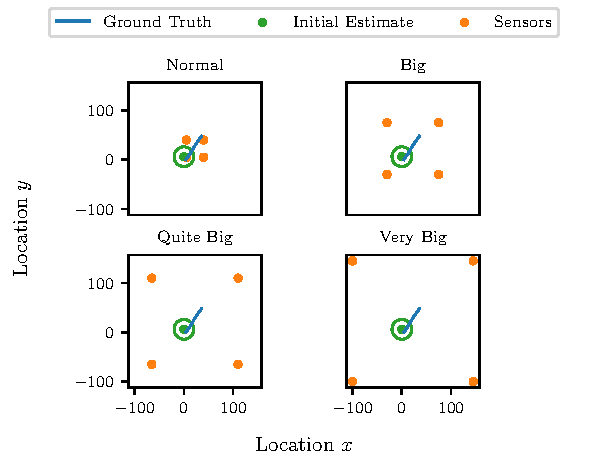
\includegraphics{figures/nonlin_fusion_simulation_layouts.pdf}
    \caption{Considered simulation layouts with varying distances between a sample navigator track and sensors.}
    \label{fig:nonlin_fusion:simulation_layouts}
\end{figure}
To demonstrate the accuracy of the method, we compared the mean square error (MSE) of the presented filter to the standard EIF using unmodified measurements. Estimation in each layout from figure \ref{fig:nonlin_fusion:simulation_layouts} consisted of $50$ filter iterations and was run $1000$ times. Unmodified measurement variances were chosen as $r_{k, i}=5$ for all $k>0$ and a large fractional precision factor, $\phi=2^{32}$, was chosen. Simulation results can be seen in figure \ref{fig:nonlin_fusion:simulation_layout_errors}.
\begin{figure}[htbp]
    \centering
    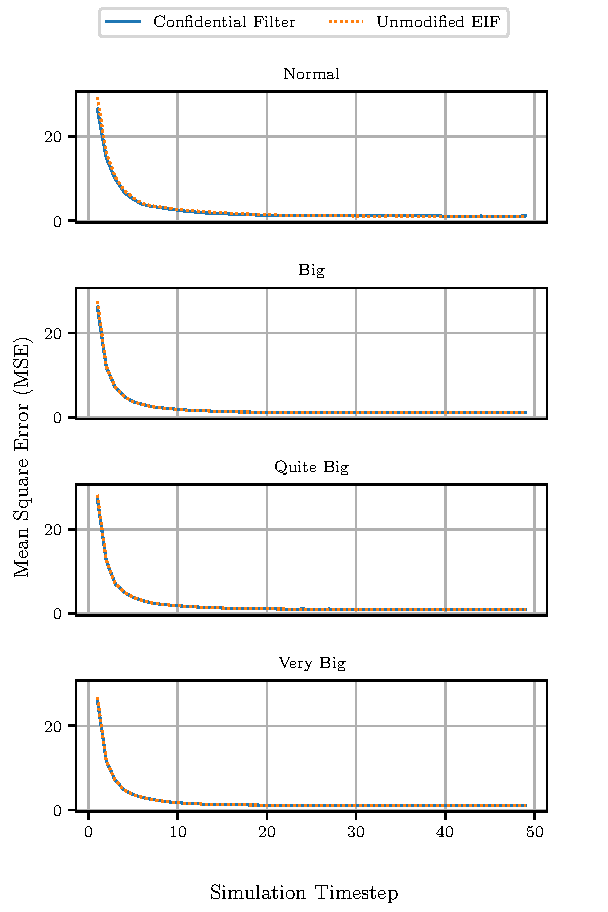
\includegraphics{figures/nonlin_fusion_simulation_layout_errors.pdf}
    \caption{Average MSE of the presented confidential filter for the different layouts over $1000$ simulation runs.}
    \label{fig:nonlin_fusion:simulation_layout_errors}
\end{figure}
From these results, we see the similarity in performance between the presented confidential localisation filter and that of the unmodified EIF. We also see that varying the distances between sensors and the navigator has little impact on the performance of the presented method. We can attribute the similar performance to the conservativeness of estimated modified measurement variances $r'_{k, i}$, eliminating additional filter divergences, and to the high fractional precision factor $\phi$, keeping computations consistent with the floating-point arithmetic of the EIF.

In addition to filter performance, computational performance is also an important factor to consider in real-time applications relying on cryptographic methods. Figure \ref{fig:nonlin_fusion:simulation_timing} shows the averages of $10$ execution times when varying the numbers of sensors and key sizes (bit lengths of $N$). Here, increasing the number of sensors primarily affected the number of inter-process communications and aggregation steps due to the asynchronous C implementation.
\begin{figure}[htbp]
    \centering
    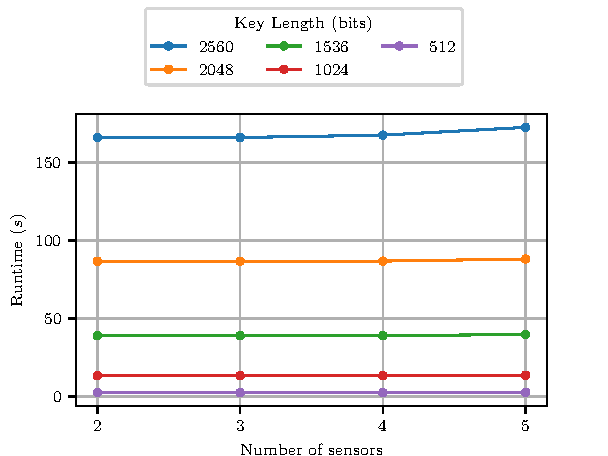
\includegraphics{figures/nonlin_fusion_simulation_timing.pdf}
    \caption{Average simulation runtimes with varying key sizes and numbers of sensors.}
    \label{fig:nonlin_fusion:simulation_timing}
\end{figure}
We can see that the predominant computational costs stem from cryptographic computations and are directly dependent on the chosen key size. In practice, choosing a key size should take into account the duration of secrecy and the secret key lifetime. For example, when relying on the DCRA for security, as is the case for the scheme presented in section \ref{sec:nonlin_fusion:lcao_scheme}, a key length of $2048$ bits is recommended for encrypting government documents \cite{barkerRecommendationPairWiseKey2019}. For our implementation and the aforementioned hardware, a $2048$ bit long key results in a filter update roughly every $1.7s$. However, if sensors are mobile and past navigations are not considered confidential, reduced key sizes may be sufficient. Further, a greater decrease in computation time may be achieved with additional code optimisations and more powerful hardware, not considered in this work.

% 
%  .d8888b.   .d88888b.  888b    888  .d8888b.  
% d88P  Y88b d88P" "Y88b 8888b   888 d88P  Y88b 
% 888    888 888     888 88888b  888 888    888 
% 888        888     888 888Y88b 888 888        
% 888        888     888 888 Y88b888 888        
% 888    888 888     888 888  Y88888 888    888 
% Y88b  d88P Y88b. .d88P 888   Y8888 Y88b  d88P 
%  "Y8888P"   "Y88888P"  888    Y888  "Y8888P"  
%                                               
%                                               
%                                               
% 

\section{Conclusions on Non-Linear Measurement Fusion with Untrusted Participants}\label{sec:nonlin_fusion:conclusion}
We have presented a localisation filter that, in the presence of range-only sensors, keeps private sensor information and navigator estimates confidential. A suitable cryptographic notion and scheme have been introduced and an implementation of the filter and scheme used to evaluate estimate and computational performance. The generalisation of the method to any non-linear measurement models fitting the form in section \ref{subsec:nonlin_fusion:solvable_nonlin_class} has been discussed, leading to a more general solution, albeit non-exhaustive, to applications in a variety of environments where sensor networks are untrusted or estimates are considered private.

Future work on the topic of confidential data fusion includes more computationally efficient schemes meeting the LCAO notion, relaxing the honest-but-curious assumption of malicious sensors and expanding the LCAO notion to enforce the consistent broadcast assumption.